\chapter{Aeolus System Overview}

This chapter presents an overview of the Aeolus security platform, on which our summarization system is based, and highlights relevant details such as log collection. More complete descriptions of the Aeolus security platform and it's log collection and analysis can be found in Cheng \cite{cheng}, Popic \cite{popic} and Blankstein \cite{blanks}.

\section{System Architecture}

\begin{figure}[ht]
\centering
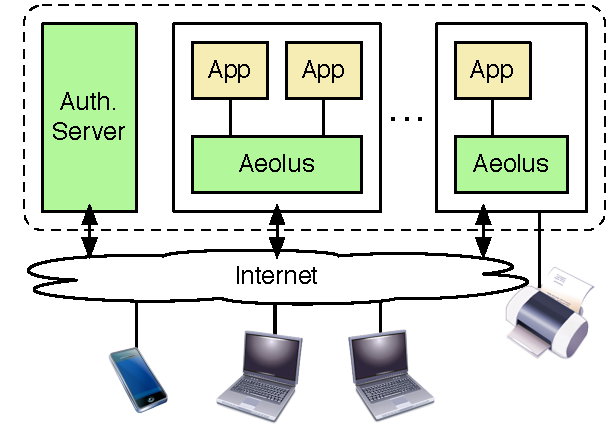
\includegraphics[bb= 0 0 292 204, width=.5\textwidth]{figures/sysarch}
\caption{High level overview of Aeolus system architecture.}
\label{fig:aeolus-sysarch}
\end{figure}

The Aeolus architecture is shown in figure \ref{fig:aeolus-sysarch}. The system consists of many nodes, each of which is trusted to enfoce Aeolus's information flow rules.

Aeolus tracks information flow within each system node and between system nodes. Nodes in the system communicate via RPC messages, those messages are encrypted to protect their secrecy and integrity. Nodes outside the system are considered to be untrusted: information can flow outside of the system if it is uncontaminated, and information arriving from the outside is marked as having no integrity.


Threads in Aeolus run on behalf of \emph{principals}. The ability of a thread to carry out \emph{privileged operations} is determined by the \emph{authority} of the principal it runs on behalf of. Aeolus tracks the authority of principals in the \emph{authority state} stored at the authority server (AS). Principals, privileged operations and authority are described in sections \ref{principals}, \ref{difc:rules} and \ref{auth} respectively.

\section{Information Flow Model}

This section describes the basic concepts and rules of the Aeolus security model.

\subsection{Prinicpals, Tags and Labels}\label{principals}

This section describes the basic concepts and rules of the Aeolus security model.

Aeolus employs an intuitive security model to implement information flow control. The model revolves around three key concepts: \emph{principals}, \emph{tags} and \emph{labels} \cite{aeolus}. Principals represent entities in the system that create, modify and share information. Tags represent security categories of information. A principal authoritative for a certain tag can modify or share information categorized by that tag. Labels are sets of tags and are used to determine whether information can flow from a source to a receiver based on the information flow rules described in the following section.

\subsection{Information Flow Rules}\label{difc:rules}

Aeolus allows information to flow from a source \emph{S} to a destination \emph{D} only if the following rules are satisfied:

\begin{eqnarray*}
  SECRECY_{S} &\subseteq& SECRECY_{D} \\
  INTEGRITY_{S} &\supseteq& INTEGRITY_{D}
\end{eqnarray*}

Threads in an Aeolus node run with security and integrity labels associated with them. In Aeolus, a thread cannot modify labels of files or shared memory objects, and hence it would have to modify it's own labels in order to read or write data. Certain label manipulations, called \emph{privileged manipulations} are unsafe because they remove constraints on information flow:

\begin{enumerate}
  \item \emph{Declassfication} Remove a tag from a secrecy label.
  \item \emph{Endorsement} Add a tag to an integrity label.
\end{enumerate}

A thread is allowed to carry out privileged label manipulatinos if it is running on behalf of a principal that has authority for the tags affected by these manipulations.

\subsection{Authority}\label{auth}

Authority determines whether a thread can perform privileged label manipulations. Authority starts with tag creation: when a thraed creates a tag, its principal has authority for that tag.

Subsequently, the Aeolus authority state can be modified through \emph{grant}, \emph{act for} or \emph{revoke} operations. Grant operations allow a principal to delegate authority for a particular tag to another principal. Act for operations allow a principal to delegate all of its authority to another principal. Revoke operations remove \emph{act for} and \emph{grant} links between principals. To avoid covert channels, Aeolus only permits threads running with null secrecy labels to modify the authority state.

\subsection{Compound Tags}

Applications frequently have sets of tags that are closely related. In order to simplify the authority structure of the application, Aeolus allows for tags to be grouped upon creation using \emph{compound tags}. For example, in a medical clinic, patient data tags are \emph{subtags} of an \emph{ALL-PATIENT-DATA} tag, a \emph{super tag}.

A principal authoritative for a super tag is also authoritative for all of its subtags. Similarly, a having super tag in a thread's secrecy label is equivalent to having all subtags in its secrecy label. This reduces label size substantially, and makes label manipulations involving paricular groups of tags less expensive.

Figure x shows a sample authority state graph, detailing \emph{act for}, \emph{grant} and \emph{subtag} relationships in the financial services application is described in chapter \ref{mint}. [describe the graph]

\section{Programming Model}

This section explains the programming abstraction Aeolus provides, and how they support DIFC.

\subsection{Threads and Vitual Nodes}

Virtual nodes, shown as applications in figure y, communicate via RPC and have many threads inside. A Virtual node is given a principal when it is created and all threads run with this principal or some prinicipal it acts for. An RPC is run in its own threads with the vn prinicipal but the labels of the claler; on the return the labels are sent back to the caller where they are merged with those of the caler: a union of the secrecy labels and an intersection of the integrity labels. Then the caller continues with its own principal.

\subsection{Shared State Objects and Boxes}\label{aeolus:shared-mem}

Within a virtual node, threads can share state via special Aeolus shared objects. Aeolus gives threads access to a \emph{root} shared memory object, which has null labels, which threads can modify to point to other Aeolus shared objects and share them.

Aeolus shared obects have immutable label associated with them, and Aeolus ensures that the rules in \ref{difc:rules} are respected. User's can create their own shared objects, however, Aeolus ensures that label manipulations do not take place inside the object's methods.

\subsection{Authority Closures and Reduced Authority Calls}
\label{aeolus:auth-calls}

Aeolus provides developers with \emph{authority closures}. An authority closure is an object bound to a principal at the moment of creation. Threads can later run the closure's methods with the closure's principal. Authority closures allow threads to allow threads to process confidential information without being exposed to the information itself.

Aeolus also provides a mechanism for threads to reduce their authority, called \emph{reduced authority calls}. To make a reduced authority call, a thread specifies a function and a principal to run it with. The calling thread's principal must act for the principal of the reduced authority call.

[labels merging?]

With those two mechanisms in place, Aeolus makes it possible to ensure that each part of the application runs with only the authority it needs. Aeolus also provides a principal that is not authoritative for any tags, \emph{P$_{PUBLIC}$}, for developers to use when they need to ensure that a part of a program cannot leak any information.

\subsection{Files}

Aeolus provides a network file system that enforces DIFC. Similarly to shared memory objects, files have immutable labels and the rules in \ref{difc:rules} apply for information flow in and out of them.

Files are yet another way (RPCs, shared memoery objects) through which Aeolus allows threads to communicate. A complete description of the Aeolus file system API is presented in McKee \cite{mckee}.

\subsection{Log Collection}

\begin{figure}[h]
\centering
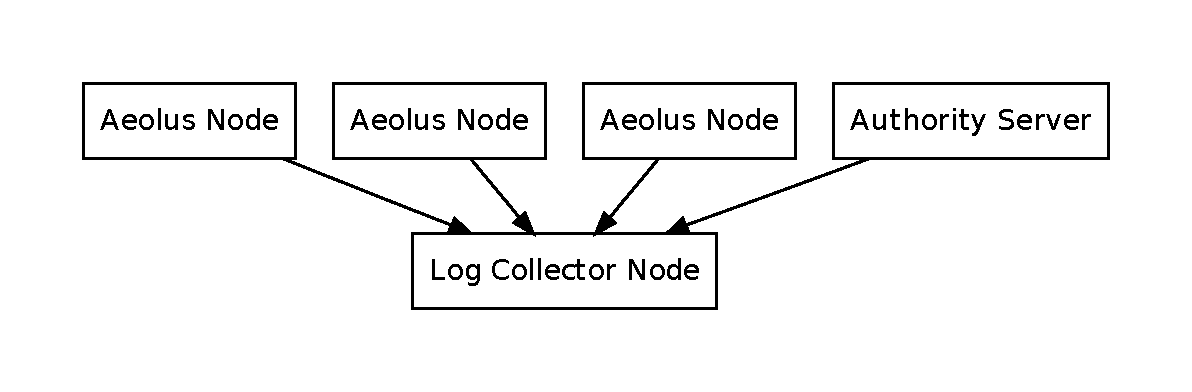
\includegraphics[height=7em]{figures/event-logging-overview}
\caption{Flow of logs to the log collection system.}
\label{fig:log-flow}
\end{figure}

Aeolus provides automatic auditing of every security related event that occurs while an application runs; also it provides a way for applications to log additional events that are meaningful at the application level.

Aeolus distributes log collection across all virtual nodes in the system. Aeolus virtual nodes send events that occur locally to the log collector as shown in figure \ref{fig:log-flow}. The log collector stores the events for later processing and analysis, as explained in \cite{blanks}. Figure y This happens automatically for all calls to the Aeolus runtime, however, Aeolus also provides application-level logging to allow developers to log their own events using the following interface:

\begin{lstlisting}[language=Java, label=app-logging]
AeolusLib.createEvent(String desc, List<String> args)
\end{lstlisting}

This creates a new record in the Aeolus event log. The \emph{desc} and \emph{args} argument are stored as attributes for that record, allowing the developer to query the event log based on the arguments they provided.

\subsubsection{Aeolus Event Attributes}

Aeolus stores different attributes for different events that take place in the system. Blankstein \cite{blanks} provides a complete description of those attributes, but here we will highlight the ones more relevant to the useof summarization:

\begin{description}
  \item[\emph{event\_counter}] \ \\
    The event counter uniquely identifies an event, and provides an
    ordering for the occurence of the event, i.e. events with a higher 
    eventcounter took place after events with a lower eventcounter.
  \item[\emph{timestamp}] \ \\
    This is the time at which the event was registered 
    by the client virtual node.
  \item[\emph{secrecy}] \ \\
    This is the secrecy label of the thread which caused the event, 
    just before the event took place.
  \item[\emph{integrity}] \ \\
    This is the integrity label of the thread which caused the event, 
    just before the event took place.
  \item[\emph{opname}] \ \\
    This field specifies the type of the event, e.g. a DECLASSIFY event, 
    or a SENDRPC event. Those types are detailed in \cite{blanks}.
    Application-level events created with the above events
    all have one opname.
  \item[\emph{app\_args}] \ \\
    This field holds the arguments specified for an application-level 
    event (the second argument in the interface shown above).
  \item[\emph{running\_principal}] \ \\
    This field holds the principal of the thread that caused the event.
\end{description}

It is important to note that the \emph{secrecy} and \emph{integrity} attributes are particularly import to prevent information leakage in the system: a thread can only read those event records if the DIFC rules in \ref{difc:rules} are satisfied.

[mention this ideally runs on david's db?]

% The audit trail is an important component of security to allow discovery of errors that cause security policies to be subverted; the audit trail can also be used to discover attacks.

%\subsection{Priviledged Operations}

%Certain label modifications are \emph{priviledged operations}: removing a tag from the secrecy label and adding a tag to the integrity label. If a process is running on behalf of a principal authoritative for a certain tag, then that process can carry priviledged operations on that tag.

%\subsection{Information Flow in and out of the System}

%Aeolus process can only write outside the system boundaries if it has empty labels. This restriction combined with the information flow rules in \ref{difc:rules} ensures that a process can only expose information if it is running on behalf of a principal authoritative for tags categorizing that information.

%Aeolus virtual nodes can use RPC to communicate with one another, and Aeolus threads can communicate using shared state mechanisms. Aeolus enforces that both of these communication mechanisms abide by the rules in \ref{difc:rules}.

%\section{Log Collection}

%Aeolus nodes are responsible for logging any events that occur locally, and sending them to the \emph{authority server} for analysis and storage.

%All calls to Aeolus runtime generate events. For example, calls that modify the authority state, or write to disk, will cause events to be logged to the system. The \emph{audit trails} system descripbed in \cite{popic} and \cite{blanks} gurantees causal relationships between events.

%The format of the event log will be described in Chapter 4.
